% \dominitoc MUST precede any \chapter
\dominitoc

% wide_margins glue — keep the cover page at the standard paper size.
% The quarto-comments extension widens \pdfpagewidth and \paperwidth at
% \AtBeginDocument (i.e. BEFORE this cover). We undo that widening here so the
% title page ships at A4, then re-apply it in template.tex AFTER \restoregeometry.
% Both registers are restored together below so TikZ's `current page` (which reads
% \paperwidth) and the physical page (\pdfpagewidth) stay consistent. /
% Glue wide_margins — garder la page de garde au format standard.
% L'extension élargit \pdfpagewidth et \paperwidth dans \AtBeginDocument (donc AVANT
% cette page de garde). On annule l'élargissement ici pour que la couverture reste en
% A4, puis on le ré-applique dans template.tex APRÈS \restoregeometry.
\ifdefined\qtcExtraMargin
  \addtolength{\pdfpagewidth}{-\qtcExtraMargin}%
  \addtolength{\paperwidth}{-\qtcExtraMargin}%
\fi

% Lowercase roman numbering for front matter (when pagestyle-sections: true)
$if(pagestyle-sections)$
\frontmatter
$endif$
\thispagestyle{empty}

% Cover page: temporary geometry, overrides the twoside layout for this page only.
% \newgeometry cannot change paper size, so it does not affect \pdfpagewidth.
% \restoregeometry after the cover brings back the twoside geometry (inner=2.5cm /
% outer=2cm); the body layout block in template.tex then finalises the TeX registers.
% Resulting \textwidth = 210 − 13 − 13 = 184 mm; tcolorbox at 165 mm fits fine. /
% Page de garde : géométrie temporaire qui surcharge le twoside pour cette page.
% \restoregeometry rétablit la géométrie twoside ; le bloc corps de template.tex
% finalise ensuite les registres TeX.
\newgeometry{
  left=13mm,
  top=15mm,
  right=13mm,
  bottom=5mm,
  nomarginpar,
  ignoreheadfoot
}

% Logos — Cnam logo flush right, co-institution logo flush left if present
\begin{minipage}{\textwidth}
$if(cotutelle)$
\hspace{0.5cm}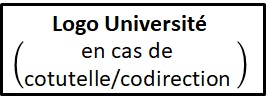
\includegraphics[width=5.5cm]{images/logo_cotut_codirec_latex.jpg}%
$endif$
\hfill
\includegraphics[width=5.5cm]{images/Cnam.jpg}
\end{minipage}

\begin{minipage}{\textwidth}
\begin{center}
\vspace{1cm}
\textbf{Conservatoire national des arts et métiers} \\
\vspace{0.5cm}
$if(ecole-doctorale)$
\textbf{ÉCOLE DOCTORALE \MakeUppercase{$ecole-doctorale$}} \\
$endif$
~\\
$if(laboratoire)$
\vspace{0.1cm}
\textbf{$laboratoire$}
\vspace{0.5cm}
$endif$
~\\
{\Huge \textbf{Thèse de doctorat}}
~\\
\vspace{0.5cm}
~\\
\text{Présentée par} : \textbf{$author$} \\
\vspace{0.1cm}
\text{Soutenue le} : \textbf{$date-soutenance$} \\
\vspace{0.1cm}
\text{Discipline} : \textbf{$discipline$} \\
\vspace{0.1cm}
\text{Spécialité} : \textbf{$specialite$} \\
\end{center}
\end{minipage}

\vspace{1cm}
\begin{center}
\begin{tcolorbox}[
  width=16.5cm,
  colback=white,
  colframe=redHESAM,
  boxrule=0.8pt,
  arc=6pt,
  left=6pt, right=6pt,
  top=4pt, bottom=4pt,
  halign=center,
]
\vspace{0.2cm}
~\\
{\LARGE\textbf{\MakeUppercase{$title$}}}
~\\
$if(subtitle)$
\vspace{0.4cm}
{\LARGE \textbf{$subtitle$}}
~\\
$endif$
\vspace{0.2cm}
\end{tcolorbox}
\end{center}
\vspace{0.8cm}

\begin{minipage}{\textwidth}
\begin{center}
\textbf{\textsc{\large Thèse dirigée par :}} \\
\vspace{0.1cm}
{\large \textbf{$directeur$}} \\
$if(codirecteur)$
\vspace{0.5cm}
\textbf{\textsc{\large et co-dirigée par :}} \\
\vspace{0.1cm}
{\large \textbf{$codirecteur$}} \\
$endif$
$if(coencadrant)$
\vspace{0.5cm}
\textbf{\textsc{\large et co-encadrée par :}} \\
\vspace{0.1cm}
{\large \textbf{$coencadrant$}} \\
$endif$
\end{center}
\end{minipage}

\vspace{0.7cm}

$if(jury)$
\noindent
\begin{minipage}{\textwidth}
% Jury table:
%   col. 1 (name, bold) and col. 3 (role) at natural width
%   col. 2 (title, institution): X — takes remaining space, wraps as needed
%   booktabs: \toprule / \bottomrule frame the table without clutter
\begin{tabularx}{\linewidth}{@{}
  >{\bfseries}l
  @{\hspace{1.5em}}
  >{\raggedright\arraybackslash}X
  @{\hspace{1.5em}}
  l
  @{}}
\toprule
\multicolumn{3}{@{}l@{}}{\textbf{Jury}} \\[2pt]
\midrule
$for(jury)$
$jury.nom$ & $jury.titre$ & $jury.role$ \\[2pt]
$endfor$
\bottomrule
\end{tabularx}
\end{minipage}
$endif$

\restoregeometry
\clearpage

% Mandatory blank page — verso of the title page
\thispagestyle{empty}
\null
\clearpage

% Dedication (optional)
$if(dedicace)$
\thispagestyle{empty}
\null\vspace{\stretch{1}}
\begin{flushright}
\itshape $dedicace$
\end{flushright}
\vspace{\stretch{2}}\null
\clearpage
$endif$
